\documentclass[discrete.tex]{subfiles}

\begin{document}
  \section{Построение транзитивного замыкания}

  \begin{reminder}[Романовский]
    Отношение транзитивно, если для любого пути в графе, соответствующему этому отношению, найдется дуга, идущая из начала пути в его конец (т.е. если любой путь "дублируется"{} соответствующий в графе дугой)
  \end{reminder}

  \begin{definition}[Григорьева]
    $G=<M,N>$ - ориентированный называется транзитивно замкнутым, если $\forall i,j \in M$, т.ч. $\e$ путь из i в j $\Ra \e$дуга u: $\Beg(u)=i,\qq \End(u)=j$
  \end{definition}

  \begin{task}
    Хотим дополнить граф так, чтобы он стал транзитивно замкнутым
  \end{task}

  \begin{Alg}[Уоршела]
    \[for\q x=1\q to\q m\q do\]
    \[\qq for\q i=1\q to\q m\q do\]
    \[\qq\qq for\q j=1\q to\q m\q do\]
    \[\qq\qq\qq if\q R[i,x]=1\q &\q R[x,y]=1\q then\q R[i,j]=1\]
  \end{Alg}

  \begin{figure}[H]
          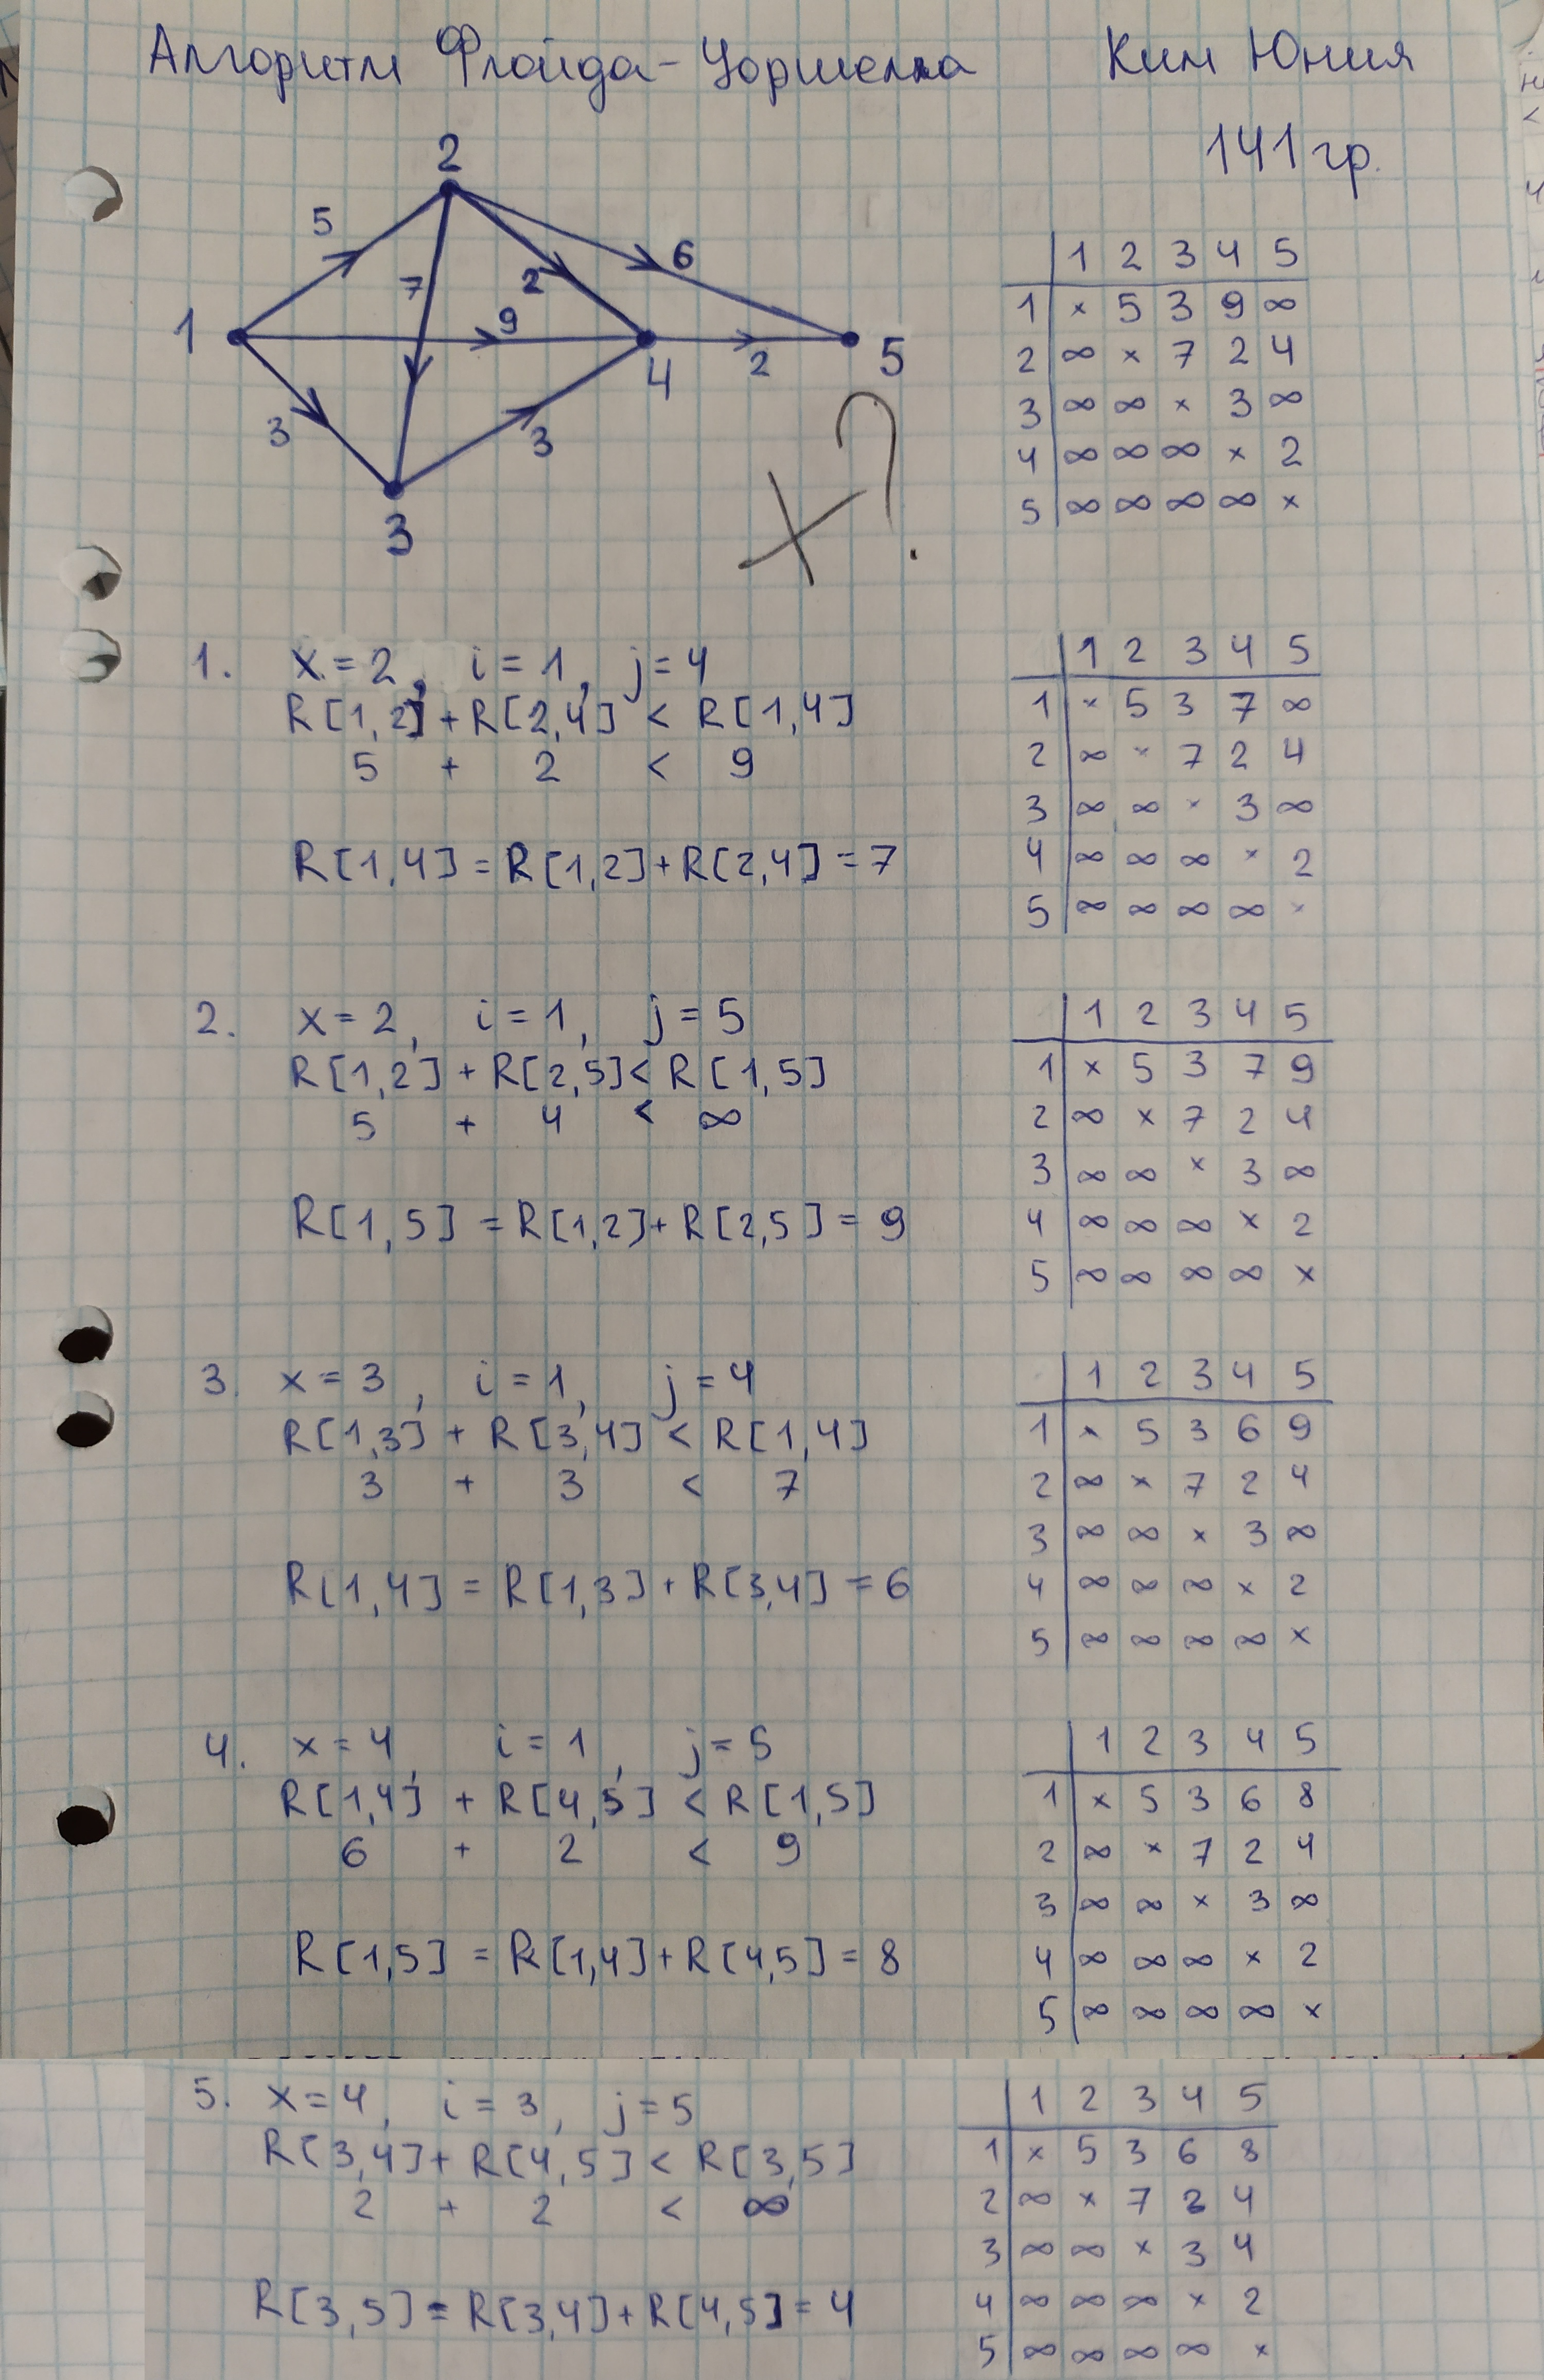
\includegraphics[width=5cm]{pics/37_2}
          \centering
  \end{figure}
\end{document}
